\documentclass{beamer}


\usepackage[frenchb]{babel}
\usepackage[T1]{fontenc}
\usepackage[utf8]{inputenc}  %\usepackage[latin1]{inputenc} selon Windows ou Ubuntu
\usepackage{multimedia}
\usepackage{url}
\usepackage{subcaption}

% Thème
\usetheme{Marburg}    %Warsaw

% Nom, titre, organisation et date
\title{Utilisation de la classification spectrale pour la caractérisation et la détection de pathologie cérébrale}
\author{Chuzel Philippe}
\institute{ENSTA Bretagne}
\date{31 aout 2016}

% Ajout du logo
\logo{
\includegraphics[height=15mm]{ensta-bretagne-vertical.png}}
\addtobeamertemplate{footline}{\insertframenumber/\inserttotalframenumber}

% Permet de parametrer la barre d'outil en verticale
%\setbeamertemplate{navigation symbols}
%{%
%\vbox{%
%\hbox{\insertslidenavigationsymbol}
%\hbox{\insertframenavigationsymbol}
%\hbox{\insertsubsectionnavigationsymbol}
%\hbox{\insertsectionnavigationsymbol}
%\hbox{\insertdocnavigationsymbol}
%\hbox{\insertbackfindforwardnavigationsymbol}}%
%}



\begin{document}



%%%%%%%%%%%%%%%%%%%%%%%%%%%%%%%%%%%%%%%%%%%%%%%%%%%%%%%%%%%%%%%%%%%%%%%%%%%%%%%%%%%%%%%%%%%%%%%%%ù


% Frame de titre
\begin{frame}
\titlepage
\end{frame}

% Permet d'imposer l'affichage du sommaire à chaque changement de section
\AtBeginSection[]
{
  \begin{frame}
  \frametitle{Sommaire}
  \tableofcontents[currentsection, hideothersubsections, pausesubsections]
  \end{frame} 
}

\section{Introduction}

% Frame 1 : expose le but du PFE
\begin{frame}

Objectif : Proposer une méthode de détection de pathologie et de segmentation automatique d'image médicale.

\begin{itemize}
\item Etude d'image IRM de perfusion.
\item Image dynamique.
\item Extraction de signal à partir de ces IRM.
\item Classification sur ces signaux.
\item Réaliser un programme de classification non-supervisé le plus automatisé possible.
\end{itemize}

\end{frame}

% Frame 2 : Montre les partenaires
\begin{frame}

Partenaires rencontrés pendant ce stage.

\begin{itemize}
\item INSERM de Lille.
\item CHRU de Brest
\end{itemize}

\begin{figure}
\centering
\begin{subfigure}[t]{0.5\textwidth}
\centering
    \vspace{0.00\textheight}
    
\includegraphics[scale=0.4,angle=0]{c34c9da0e3.jpg}
    \label{fig:CHRU} 
\end{subfigure}
\begin{subfigure}[t]{0.5\textwidth}
\centering
    \vspace{0.00\textheight}
    
\includegraphics[scale=0.2,angle=0]{inserm_logo.jpg}
    \label{fig:Inserm} 
\end{subfigure}
    \label{fig:Partenaires} 
\end{figure}

\end{frame}



%%%%%%%%%%%%%%%%%%%%%%%%%%%%%%%%%%%%%%%%%%%%%%%%%%%%%%%%%%%%%%%%%%%%%%%%%%%%%%%%%%%%%%%%%%%%%%%%%ù

\section{Évolution du PFE.}


% Frame 1
\begin{frame}
\frametitle{Introduction}

Sujet étudié actuellement à l'ENSTA Bretagne :

\bigskip 

\begin{Large}
\textcolor{blue}{"Détection et caractérisation de la thrombose"}
\end{Large}

\bigskip 

La piste utilisant des images d'élastométrie et d'échographie est étudier par M. Thibaud Berthomier, en thèse actuellement à l'ENSTA Bretagne.

\end{frame}

% Frame 2
\begin{frame}
\frametitle{Introduction}

Premier sujet proposé par M. Ali Mansour:

\bigskip 

\begin{Large}
\textcolor{blue}{"Étudier la piste des IRM pour la détection et la caractérisation de la thrombose."}
\end{Large}

\end{frame}

% Frame 3
\begin{frame}[allowframebreaks]

Listes des problèmes rencontrés pendant l'étude:
\begin{itemize}
\item Signature extrêmement variable avec le temps
\item Déplacement du caillot au cours du temps
\item le type et la composition du caillot ne peut être déduits ssi on extrait le caillot.
\end{itemize}

\end{frame}

% Frame 4
\begin{frame}[allowframebreaks]

\bigskip

$\rightarrow$ Redirection du projet de fin d'étude.

\bigskip
Proposition de M.Gentrix: 

\bigskip

\begin{Large}
\textcolor{blue}{Application vers la caractérisation et la détection de pathologie cérébrale.}
\end{Large}

$\rightarrow$ Tentative de publication d'article au cours du mois de juin.

\end{frame}

%%%%%%%%%%%%%%%%%%%%%%%%%%%%%%%%%%%%%%%%%%%%%%%%%%%%%%%%%%%%%%%%%%%%%%%%%%%%%%%%%%%%%%%%%%%%%%%%%ù

\section{Méthodologie.}


% Frame 1
\begin{frame}

Après deux mois de travail principalement bibliographique, nous avons pu récupérer deux sources d'images :

\begin{itemize}
\item Images IRM de pathologie prostatique de l'INSERM de Lille qui a été le premier a implémenté la classification spectrale pour l'aide au diagnostic.
\item Images d'IRM de cerveau présentant certaines pathologies fournies par le CHRU de Brest.
\item Proposition de la part du HIA Clermont Tonnerre mais qui n'a pas aboutie.
\end{itemize}

\end{frame}

% Frame 2
\begin{frame}

Au final, nous avons pu établir une base de données de d'image IRM de cerveau de 13 patients présentant toutes une pathologie :

\begin{itemize}
\item Tumeur.
\item Hématome.
\item ...
\end{itemize} 

On arrive a des ensembles d'image de taille 128*128 pixels qui traduisent la diffusion d'un produit de contraste dans les tissus cérébraux.

\end{frame}

\begin{frame}

\begin{figure}

\frametitle{Chaine de traitement développé dans le cadre du PFE.}
\centering
    \includegraphics[scale=0.5,angle=0]{Processing_toolchain.png}
    \label{fig:Chaine} 
    
\end{figure}

\end{frame}

%%%%%%%%%%%%%%%%%%%%%%%%%%%%%%%%%%%%%%%%%%%%%%%%%%%%%%%%%%%%%%%%%%%%%%%%%%%%%%%%%%%%%%%%%%%%%%%%%ù

\section{La classification spectrale.}

\begin{frame}[allowframebreaks]
Idée: proposer un algorithme non-supervisé qui pourrait réaliser des clusters à partir des informations extraites de ces images.

$\rightarrow$ Extraction de signaux temporels correspondant à l'évolution d'intensité d'un pixel donné.

\begin{figure}
\centering
    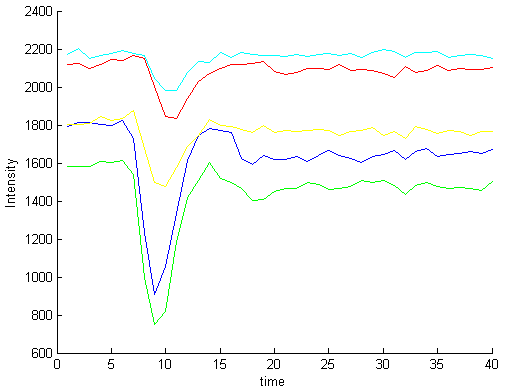
\includegraphics[scale=0.5,angle=0]{CourbeExample.png}
    \label{fig:Courbe} 
\end{figure}

\end{frame}

\begin{frame}

\textcolor{red}{Problème:}

\medskip

Les algorithmes classiques de classification non-supervisée comme le k-means ne sont pas adaptés pour la classification de signaux temporels.

\medskip

\textcolor{blue}{Proposition:}

\medskip

Utiliser la classification spectrale qui a déjà été employé pour ce type de données.

\end{frame}

\begin{frame}

\textcolor{blue}{Principe:}

\medskip
Se placer dans un espace plus adapté pour la classification.

\medskip

\textcolor{blue}{Principales étapes:}

\begin{itemize}
\item Construction d'un graphe sur toutes les données.
\item Construction d'une matrice de voisinage qui traduit la proximité des données entre elles.
\item Travail de classification sur les vecteurs propres et valeurs propres de cette matrice.
\end{itemize}

\end{frame}

\begin{frame}

\textcolor{blue}{Construction du graphe:}

\begin{itemize}
\item Graphe entièrement connecté.
\item Construction de la matrice de similarité noté W.
\end{itemize}

\begin{figure}
\centering
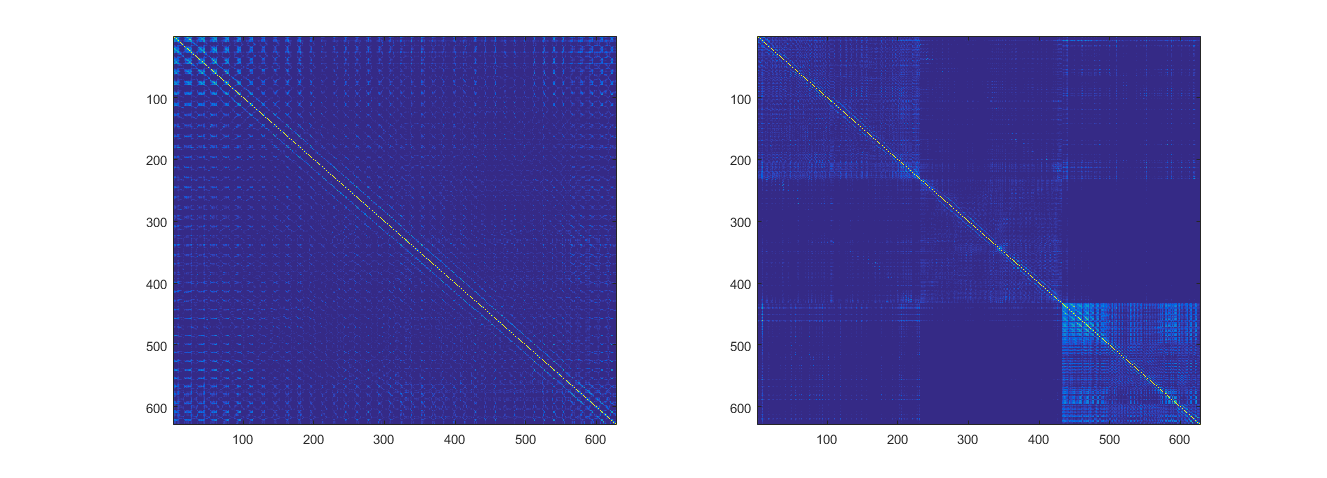
\includegraphics[scale=0.27,angle=0]{L.png}
\label{fig:MA} 
\end{figure}

\end{frame}

\begin{frame}

Calcul de la matrice Laplacienne $L$ de $W$ défini par la formule 


\begin{equation}
\centering
L = I - D^{1/2} W D^{1/2}
\end{equation}

Où D est la matrice de degrés défini par $d_{ii} = \sum_j w_{ij}$, une matrice diagonale et $I$ est la matrice identité.

\medskip

On va ensuite extraire les vecteurs propres associés aux plus petites valeurs propres de la matrice $L$ et on crée des clusters à partir des informations portées par ces vecteurs propres.

\end{frame}

\begin{frame}

Exemple d'application:

\begin{figure}
\centering
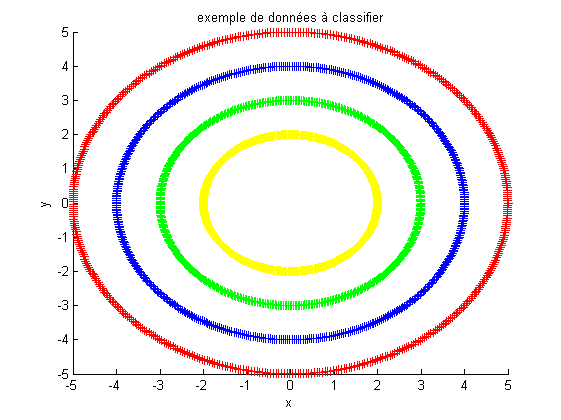
\includegraphics[scale=0.5,angle=0]{DataSet.png}
\label{fig:MA} 
\end{figure}

\end{frame}

\begin{frame}

Résultats des k-means:

\begin{figure}
\centering
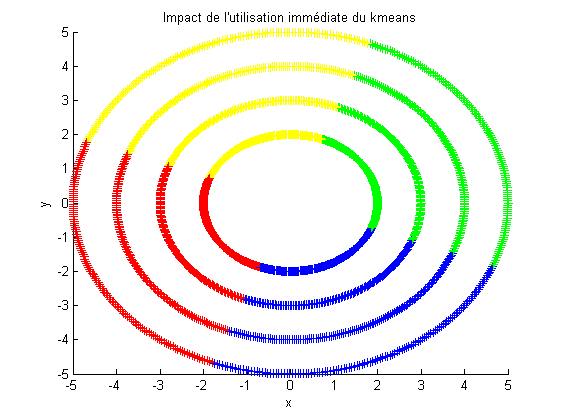
\includegraphics[scale=0.5,angle=0]{AlgoKmeans.png}
\label{fig:MA} 
\end{figure}

\end{frame}

\begin{frame}

Résultats de l'algorithme de classification spectrale:

\begin{figure}
\centering
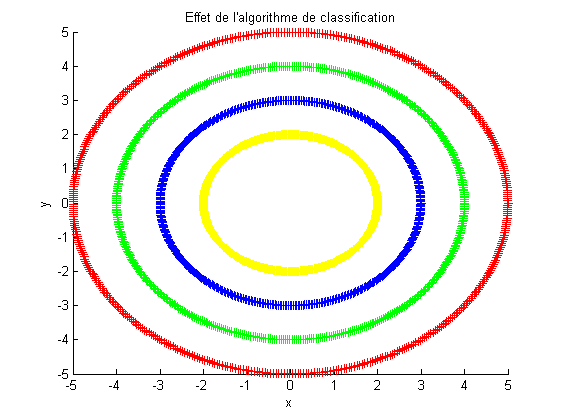
\includegraphics[scale=0.5,angle=0]{AlgoClssification.png}
\label{fig:MA} 
\end{figure}

\end{frame}

\begin{frame}

\begin{figure}

\frametitle{Chaine de traitement développé dans le cadre du PFE.}
\centering
    \includegraphics[scale=0.5,angle=0]{Processing_toolchain.png}
    \label{fig:Chaine} 
    
\end{figure}

\end{frame}



%%%%%%%%%%%%%%%%%%%%%%%%%%%%%%%%%%%%%%%%%%%%%%%%%%%%%%%%%%%%%%%%%%%%%%%%%%%%%%%%%%%%%%%%%%%%%%%%%ù

% Résultats.

\section{Résultats.}

\begin{frame}

Présentation des résultats des algorithmes pour deux patients:

\begin{itemize}
\item Une patiente présentant un cancer.
\item Un patient présentant un lymphome cérébrale primitive.
\end{itemize}

\url{IRMsain.avi}


\end{frame}

% Frame 1 résultat patient 2
\begin{frame}

\url{videoOut17.avi}

\end{frame}

\begin{frame}

% Frame 1 résultat patient 4
Résultats du programme sur les IMRs récupérées:
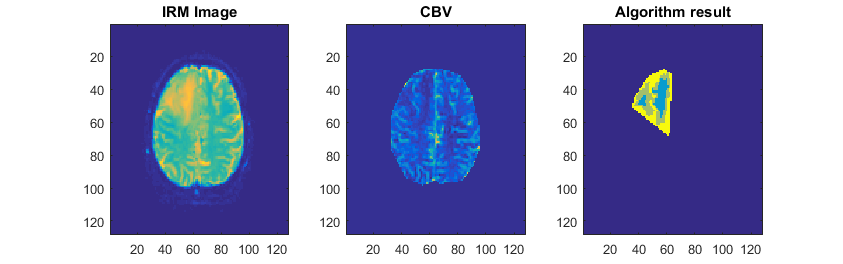
\includegraphics[scale=0.40]{Patient2Result.png}

Ici, on voit clairement 2 principaux tissus:
\begin{itemize}
\item Une protubérance à gauche qui correspond à une tumeur et un œdème.
\item le tissu sain.
\end{itemize}
\end{frame}

\begin{frame}
\centering
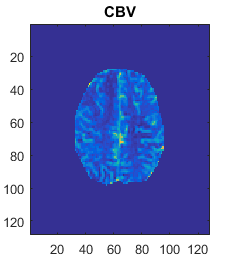
\includegraphics[scale=0.80]{Patient2Result-CBV.png}

\end{frame}

\begin{frame}
\centering
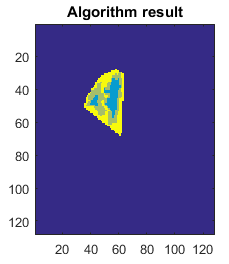
\includegraphics[scale=0.80]{Patient2Result-ALGO.png}

\end{frame}

% Frame 1 résultat patient 4

\begin{frame}

\url{videoOut13.avi}

\end{frame}

\begin{frame}

Résultats du programme sur les IMRs récupérées:
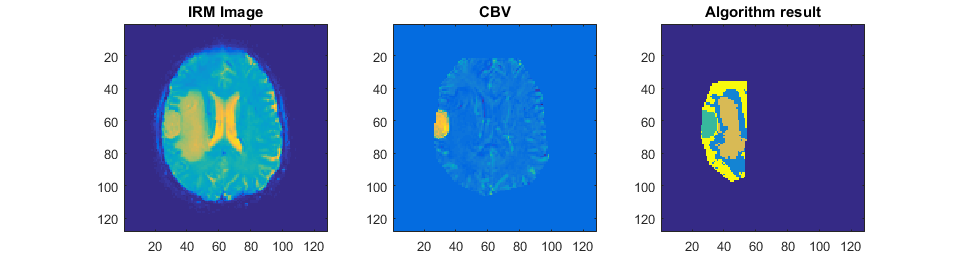
\includegraphics[scale=0.40]{Patient4Result.png}

Ici, on voit clairement quatre principaux tissus:
\begin{itemize}
\item Une protubérance à gauche qui correspond à une tumeur ici bénigne.
\item La zone à sa droite qui correspond à un hématome.
\item Le ventricule cérébral au centre.
\item le tissu sain.
\end{itemize}
\end{frame}

\begin{frame}
\centering

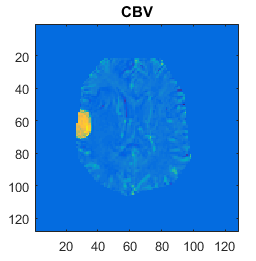
\includegraphics[scale=0.8]{Patient4Result-CBV.png}

\end{frame}

\begin{frame}
\centering

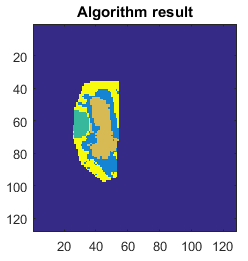
\includegraphics[scale=0.8]{Patient4Result-ALGO.png}

\end{frame}

% Conclusion

\begin{frame}

\textcolor{red}{Conclusion:}

\begin{itemize}
\item Méthode particulièrement adaptée pour certaines pathologies qui impacte la vascularisation et la diffusion du produit de contrast.
\item Permet d'isoler facilement les pathologies et autres symptômes comme les œdèmes des tissus sains.
\end{itemize}

Néanmoins:

\begin{itemize}
\item Pour certaines maladies, il faut avoir recours à d'autres méthodes (CBV, autres modalités d'IRM ...)
\item Besoin d'une connaissance a priori sur la ROI à sélectionner.
\end{itemize}


\end{frame}

%%%%%%%%%%%%%%%%%%%%%%%%%%%%%%%%%%%%%%%%%%%%%%%%%%%%%%%%%%%%%%%%%%%%%%%%%%%%%%%%%%%%%%%%%%%%%%%%%ù

% Remerciment + Question

\begin{frame}

Un immense remerciement:

\begin{itemize}
\item Ali Mansour et Thibaud Berthomier à l'ENSTA Bretagne.
\item Jean-Christophe Gentrix et Julien Ognard au CHRU de Brest, Cavale Blanche.
\item Nacim Betrouni et Denis Hamad à l'INSERM de Lille.
\end{itemize}

\end{frame}

\begin{frame}

\begin{center}
\textcolor{blue}{\Huge Des Questions ?}
\end{center}

\end{frame}

\end{document}
